\documentclass[journal]{IEEEtran}

\usepackage{cite}
\usepackage{amsmath,amssymb,amsfonts}
\usepackage{graphicx}
\usepackage{textcomp}
\usepackage{xcolor}
\usepackage{booktabs}
\usepackage{multirow}
\usepackage{array}
\usepackage{url}
\usepackage[hidelinks]{hyperref}

\setcounter{dbltopnumber}{4}
\renewcommand{\dbltopfraction}{0.92}
\renewcommand{\textfraction}{0.06}
\renewcommand{\floatpagefraction}{0.85}
\renewcommand{\dblfloatpagefraction}{0.85}

\begin{document}

\title{Comparative Evaluation of Tree-Based, Ensemble, and Margin Classifiers for Early Diabetes Mellitus Prediction Under Zero-Leakage Preprocessing and Class Imbalance}

\author{Mokhammad~Dwi~Nurkolis%
\thanks{Manuscript prepared on November 20, 2026. This experimental study was conducted as part of the graduate course in Machine Learning (Pembelajaran Mesin), Master of Informatics Program, Faculty of Industrial Technology, Universitas Islam Indonesia, Yogyakarta, Indonesia.}%
\thanks{Mokhammad Dwi Nurkolis (Student ID / NIM: 26917015) is with the Master of Informatics Program, Faculty of Industrial Technology, Universitas Islam Indonesia, Yogyakarta 55584, Indonesia (e-mail: halo@nurkolis.xyz).}}

\markboth{IEEE JOURNAL ARTICLE DRAFT --- MASTER OF INFORMATICS, UNIVERSITAS ISLAM INDONESIA, NOVEMBER 2026}%
{Nurkolis: Comparative Evaluation of Machine Learning Classifiers for Early Diabetes Prediction}

\maketitle

\begin{abstract}
Early and reliable screening of Type 2 Diabetes Mellitus (T2DM) from routine clinical measurements is critical for preventing irreversible microvascular and macrovascular complications. However, developing trustworthy machine learning (ML) models on clinical tabular datasets such as the Pima Indians Diabetes Database ($N = 768$) is frequently compromised by three methodological pitfalls: (1) unaddressed biologically impossible zero values masquerading as valid measurements, (2) severe sensitivity degradation caused by class imbalance ($65.1\%$ non-diabetic vs.\ $34.9\%$ diabetic), and (3) optimistic performance inflation due to preprocessing data leakage prior to cross-validation splitting. In this study, we conduct a rigorous three-stage experimental benchmark comparing four distinct algorithmic paradigms: Decision Tree (CART), Random Forest (bagging ensemble), Extreme Gradient Boosting (XGBoost, second-order boosting), and Support Vector Machine (SVM with radial basis function kernel). All transformations---converting physiological zeroes in Glucose, Blood Pressure, Skin Thickness, Insulin, and Body Mass Index (BMI) to missing indicators, median imputation, z-score standardization, and Synthetic Minority Over-sampling Technique (SMOTE)---are strictly encapsulated within fold-internal training pipelines. Empirical results on the held-out stratified test set ($N = 154$) reveal that baseline models achieve high specificity ($0.7900$--$0.8600$) but clinically inadequate sensitivity ($0.4815$--$0.6111$) and exhibit severe overfitting in unregularized tree models (train-to-test F1 gaps of $0.3465$--$0.4851$). Integrating fold-internal SMOTE and 5-fold stratified hyperparameter optimization elevates minority-class sensitivity to $0.7407$--$0.7963$ while compressing generalization gaps below $0.16$. Tuned XGBoost achieves the highest overall discriminative ranking performance (5-fold CV F1 $= 0.7121 \pm 0.0209$, Test ROC-AUC $= 0.8224$, PR-AUC $= 0.7125$, Sensitivity $= 0.7778$, Specificity $= 0.7100$), whereas the regularized Decision Tree ($\text{max\_depth}=4$, $\text{min\_samples\_leaf}=15$) yields the highest point-estimate test F1-score ($0.7049$, Sensitivity $= 0.7963$, Specificity $= 0.7500$) with a minimal train-test F1 gap of $0.0165$.
\end{abstract}

\begin{IEEEkeywords}
Diabetes mellitus prediction, bias--variance trade-off, class imbalance, data leakage prevention, decision tree, random forest, SMOTE, support vector machine, XGBoost.
\end{IEEEkeywords}

\section{Introduction}
\IEEEPARstart{D}{iabetes} Mellitus (DM) is a chronic metabolic disorder characterized by persistent hyperglycemia resulting from defects in insulin secretion, insulin action, or both. Left undiagnosed or inadequately managed, Type 2 Diabetes Mellitus (T2DM) leads to progressive damage across major organ systems, including diabetic retinopathy, nephropathy, peripheral neuropathy, and cardiovascular disease \cite{smith1988using, zou2018predicting}. Because early-stage T2DM is frequently asymptomatic, non-invasive clinical decision support systems capable of stratifying patient risk from routine demographic and physiological variables offer substantial value for clinical triage and preventive intervention \cite{maniruzzaman2020classification}.

Despite extensive literature applying machine learning (ML) classifiers to clinical tabular benchmarks such as the National Institute of Diabetes and Digestive and Kidney Diseases (NIDDK) Pima Indians Diabetes Database \cite{smith1988using, sisodia2018prediction}, translating reported accuracies into clinical reliability remains challenging. A critical audit of published experimental workflows reveals three recurring methodological flaws:

\begin{enumerate}
    \item \emph{Disguised Missing Data (Biologically Impossible Zeroes):} In the canonical Pima dataset ($N = 768$), missing clinical measurements were historically encoded as numerical zeroes ($0$). In living human patients, values of zero for plasma glucose concentration, diastolic blood pressure, triceps skinfold thickness, 2-hour serum insulin, or body mass index (BMI) are physiologically impossible. Treating these zeroes as true numerical observations severely distorts decision boundaries, kernel distances, and feature correlations.
    \item \emph{Preprocessing and Resampling Data Leakage:} Numerous prior studies perform imputation, feature scaling, or Synthetic Minority Over-sampling Technique (SMOTE) across the entire dataset \emph{prior} to train-test splitting or cross-validation \cite{kaufman2012leakage, kapoor2023leakage}. When synthetic minority samples are generated globally before partitioning, near-duplicate interpolated vectors appear simultaneously in both training and evaluation splits, artificially inflating reported sensitivity and F1-scores while failing to generalize to unseen patients.
    \item \emph{Accuracy Paradox Under Class Imbalance and Neglect of Bias--Variance Diagnostics:} With $65.10\%$ non-diabetic ($n = 500$) and $34.90\%$ diabetic ($n = 268$) instances, a classifier optimizing standard empirical risk favors the majority class, yielding high specificity but unacceptably high false-negative rates (low sensitivity/recall) \cite{he2009learning}. Furthermore, unconstrained tree-based learners easily memorize small clinical cohorts ($F_{1,\text{train}} = 1.0000$), yet many studies report only single-point test accuracy without evaluating train-versus-validation learning curves or bias--variance dynamics.
\end{enumerate}

To address these gaps, this study formulates three explicit research questions:
\begin{itemize}
    \item \textbf{RQ1 (Algorithmic Paradigm Comparison):} How do single decision trees (CART), bagging ensembles (Random Forest), gradient-boosted trees (XGBoost), and margin-based kernel classifiers (SVM) compare in balancing sensitivity and specificity under a strict zero-leakage preprocessing pipeline?
    \item \textbf{RQ2 (Quantifiable Improvement via Imbalance Handling and Regularization):} To what extent do fold-internal SMOTE resampling and stratified hyperparameter tuning improve minority-class recall and F1-score compared to unadjusted baseline models?
    \item \textbf{RQ3 (Bias--Variance Characterization):} How do structural regularization constraints (tree depth pruning, minimum leaf sample thresholds, $L_2$ weight shrinkage, and SVM margin regularization) alter the bias--variance trade-off across sample sizes?
\end{itemize}

The remainder of this paper is organized as follows. Section~II reviews related work on clinical diabetes classification and leakage-free evaluation protocols. Section~III details the dataset audit, zero-leakage pipeline architecture, algorithmic formulations, and three-stage experimental design. Section~IV presents the empirical results, confusion matrix analyses, ROC/PR curves, learning curve diagnostics, and clinical feature attribution. Section~V concludes the study.

\section{Related Work}
The Pima Indians Diabetes cohort was originally introduced by Smith \emph{et al.}\ \cite{smith1988using} to evaluate the ADAP adaptive learning routine, achieving a sensitivity and specificity of $76\%$ on a split of 576 training and 192 test cases. Since its inclusion in the UCI and OpenML repositories, the dataset has served as a foundational benchmark for supervised classification.

Sisodia and Sisodia \cite{sisodia2018prediction} compared Naive Bayes, Decision Tree, and Support Vector Machine (SVM) classifiers on the Pima dataset, reporting a peak accuracy of $76.30\%$ with Naive Bayes. However, their evaluation did not replace biologically invalid zeroes prior to modeling and relied primarily on overall accuracy and ROC-AUC without addressing the $1:1.87$ class imbalance or quantifying false-negative error rates in detail.

Zou \emph{et al.}\ \cite{zou2018predicting} evaluated Decision Tree (J48), Random Forest, and Neural Networks on both the Pima dataset and a hospital physical examination cohort from Luzhou, China, applying Principal Component Analysis (PCA) and Minimum Redundancy Maximum Relevance (mRMR) feature selection. They demonstrated that Random Forest outperformed single decision trees (reaching $77.21\%$ accuracy on Pima) and identified fasting/plasma glucose as the dominant predictor, though class-imbalance resampling and learning-curve variance diagnostics were not systematically isolated.

Maniruzzaman \emph{et al.}\ \cite{maniruzzaman2020classification} investigated median-based missing value replacement combined with Random Forest feature selection and multiple classifiers (Naive Bayes, Decision Tree, AdaBoost, and Random Forest), demonstrating that replacing biological zeroes with group medians substantially improved classification stability. Nevertheless, recent methodological audits by Kaufman \emph{et al.}\ \cite{kaufman2012leakage} and Kapoor and Narayanan \cite{kapoor2023leakage} emphasize that any imputation statistics or oversampling transformations (such as SMOTE \cite{chawla2002smote}) computed across the full dataset before cross-validation introduce severe data leakage.

Table~\ref{tab:related_work} summarizes representative studies and contrasts their methodological protocols with our experimental framework. Unlike prior works that evaluate single hyperparameter configurations or permit global preprocessing, our study enforces fold-internal pipeline isolation across three progressive experimental stages and explicitly quantifies the bias--variance trade-off via cross-validated learning curves.

\begin{table*}[t]
\centering
\caption{Comparison of Related Machine Learning Studies on Diabetes Mellitus Classification and Methodological Rigor}
\label{tab:related_work}
\begin{tabular}{p{2.7cm}p{2.8cm}p{2.5cm}p{2.3cm}p{2.3cm}p{3.2cm}}
\toprule
\textbf{Study / Reference} & \textbf{Algorithms Evaluated} & \textbf{Biological Zero Handling} & \textbf{Imbalance Strategy} & \textbf{Zero-Leakage CV Pipeline} & \textbf{Bias--Variance \& Metric Scope} \\
\midrule
Smith \emph{et al.}\ (1988) \cite{smith1988using} & ADAP Neural Routine & Raw encoding retained & None & Hold-out split ($576 / 192$) & Sensitivity \& Specificity ($0.76$); no F1 or learning curves \\
Sisodia \& Sisodia (2018) \cite{sisodia2018prediction} & Naive Bayes, Decision Tree, SVM & Raw zeroes retained & None & 10-fold CV (global) & Accuracy ($76.3\%$), Precision, Recall, F1, ROC-AUC \\
Zou \emph{et al.}\ (2018) \cite{zou2018predicting} & J48 Decision Tree, Random Forest, ANN & Pre-filtered / mRMR \& PCA & None & 5-fold CV & Accuracy ($77.2\%$), Sensitivity, Specificity, MCC \\
Maniruzzaman \emph{et al.}\ (2020) \cite{maniruzzaman2020classification} & NB, DT, AdaBoost, Random Forest & Median imputation & None & 10-fold CV & Accuracy, Sensitivity, Specificity, ROC-AUC \\
\textbf{This Study (2026)} & \textbf{Decision Tree, Random Forest, XGBoost, SVM} & \textbf{Fold-internal Zero$\to$NaN + Median Imputation} & \textbf{Fold-internal SMOTE + GridSearch} & \textbf{Strict \texttt{imblearn} Pipeline in 5-Fold CV} & \textbf{Acc, Prec, Sens, Spec, F1, G-Mean, ROC/PR-AUC, 95\% CI, Learning Curves} \\
\bottomrule
\end{tabular}
\end{table*}

\section{Methodology}

\subsection{Dataset Characteristics and Biological Zero Audit}
We utilize the canonical Pima Indians Diabetes Database retrieved from OpenML (Data ID 37, originally compiled by the NIDDK) \cite{smith1988using}. The cohort comprises $N = 768$ female patients of Pima Indian heritage aged 21 years and older residing near Phoenix, Arizona. Each patient record consists of $d = 8$ numeric clinical attributes and a binary diagnostic target $y \in \{0, 1\}$, where $y = 1$ denotes a positive T2DM diagnosis within five years according to World Health Organization (WHO) criteria (2-hour post-load plasma glucose $\ge 200\text{ mg/dL}$).

As illustrated in Fig.~\ref{fig:eda_audit}(a), the target distribution exhibits moderate class imbalance: $500$ patients ($65.10\%$) tested negative ($y = 0$) and $268$ patients ($34.90\%$) tested positive ($y = 1$), corresponding to an imbalance ratio of $1 : 1.8657$.

A critical data quality inspection reveals that while the raw dataset contains zero explicit \texttt{NULL} entries, five physiological variables contain biologically impossible zero values ($0$):
\begin{itemize}
    \item \textbf{2-Hour Serum Insulin ($\mu\text{U/mL}$):} $374$ zero entries ($48.70\%$ missingness).
    \item \textbf{Triceps Skinfold Thickness ($\text{mm}$):} $227$ zero entries ($29.56\%$ missingness).
    \item \textbf{Diastolic Blood Pressure ($\text{mm Hg}$):} $35$ zero entries ($4.56\%$ missingness).
    \item \textbf{Body Mass Index ($\text{kg/m}^2$):} $11$ zero entries ($1.43\%$ missingness).
    \item \textbf{Plasma Glucose Concentration ($\text{mg/dL}$):} $5$ zero entries ($0.65\%$ missingness).
\end{itemize}
By contrast, a value of $0$ for \emph{Pregnancies} is biologically valid, and neither \emph{Diabetes Pedigree Function} nor \emph{Age} contains zero values. Table~\ref{tab:dataset_audit} details the distributional shift before and after recoding these invalid zeroes as missing values (\texttt{NaN}). Notably, the raw mean of Serum Insulin is artificially depressed to $79.80 \pm 115.24\text{ }\mu\text{U/mL}$, whereas the valid physiological distribution has a mean of $155.55 \pm 118.78\text{ }\mu\text{U/mL}$ and a median of $125.00\text{ }\mu\text{U/mL}$ (interquartile range, $\text{IQR} = 113.75$). Because physiological features such as Insulin and Skin Thickness exhibit right-skewed distributions with extreme outliers (Fig.~\ref{fig:corr_box}(b)), median imputation is selected over mean imputation for robustness.

\begin{table*}[t]
\centering
\caption{Clinical Feature Schema and Biologically Impossible Zero Audit of the Pima Indians Diabetes Cohort ($N = 768$)}
\label{tab:dataset_audit}
\resizebox{\textwidth}{!}{%
\begin{tabular}{llrrrrrrr}
\toprule
\textbf{Feature Name} & \textbf{Clinical Unit / Description} & \textbf{Raw Mean $\pm$ SD} & \textbf{Raw Range} & \textbf{Invalid $0$ ($n$)} & \textbf{Invalid $0$ (\%)} & \textbf{Valid Median (IQR)} & \textbf{Valid Mean $\pm$ SD} \\
\midrule
\texttt{Pregnancies} & Number of times pregnant (count) & $3.85 \pm 3.37$ & $[0.0, 17.0]$ & $0^*$ & $0.00\%$ & $3.00$ ($5.00$) & $3.85 \pm 3.37$ \\
\texttt{Glucose} & 2-hr OGTT plasma glucose ($\text{mg/dL}$) & $120.89 \pm 31.97$ & $[0.0, 199.0]$ & $5$ & $0.65\%$ & $117.00$ ($42.00$) & $121.69 \pm 30.54$ \\
\texttt{BloodPressure} & Diastolic blood pressure ($\text{mm Hg}$) & $69.11 \pm 19.36$ & $[0.0, 122.0]$ & $35$ & $4.56\%$ & $72.00$ ($16.00$) & $72.41 \pm 12.38$ \\
\texttt{SkinThickness} & Triceps skinfold thickness ($\text{mm}$) & $20.54 \pm 15.95$ & $[0.0, 99.0]$ & $227$ & $29.56\%$ & $29.00$ ($14.00$) & $29.15 \pm 10.48$ \\
\texttt{Insulin} & 2-hr serum insulin ($\mu\text{U/mL}$) & $79.80 \pm 115.24$ & $[0.0, 846.0]$ & $374$ & $48.70\%$ & $125.00$ ($113.75$) & $155.55 \pm 118.78$ \\
\texttt{BMI} & Body mass index ($\text{kg/m}^2$) & $31.99 \pm 7.88$ & $[0.0, 67.1]$ & $11$ & $1.43\%$ & $32.30$ ($9.10$) & $32.46 \pm 6.92$ \\
\texttt{DiabetesPedigree} & Genetic diabetes pedigree function & $0.47 \pm 0.33$ & $[0.08, 2.42]$ & $0$ & $0.00\%$ & $0.37$ ($0.38$) & $0.47 \pm 0.33$ \\
\texttt{Age} & Patient age (years) & $33.24 \pm 11.76$ & $[21.0, 81.0]$ & $0$ & $0.00\%$ & $29.00$ ($17.00$) & $33.24 \pm 11.76$ \\
\bottomrule
\multicolumn{8}{l}{\footnotesize $^*$A value of $0$ for \texttt{Pregnancies} represents nulliparity (biologically valid) and is therefore preserved without imputation.}
\end{tabular}%
}
\end{table*}

\begin{figure*}[t]
\centering
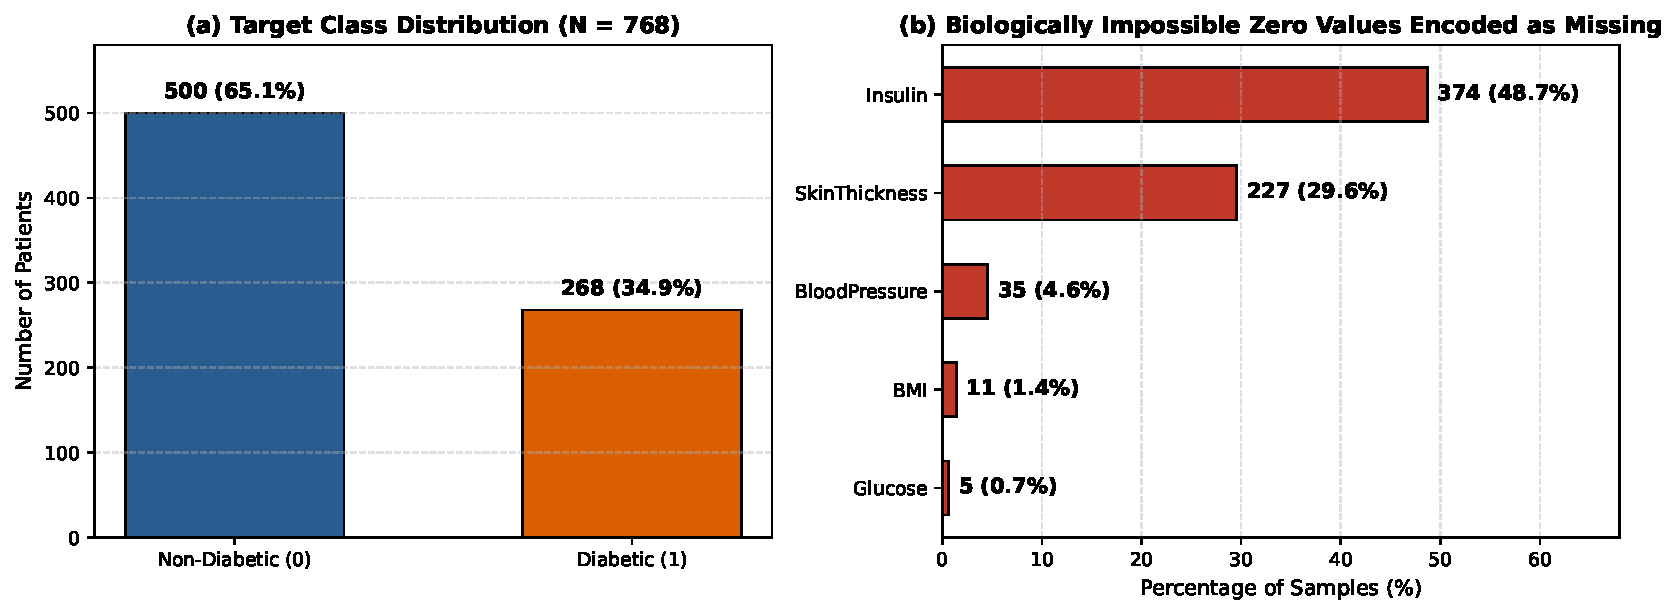
\includegraphics[width=0.84\textwidth]{../artifacts/figures/fig1_class_and_missing_audit.pdf}
\caption{Exploratory data audit of the Pima Indians Diabetes cohort ($N = 768$): (a) target class distribution demonstrating a $65.1\%$ ($n=500$) to $34.9\%$ ($n=268$) class imbalance ratio ($1:1.87$); (b) prevalence of biologically impossible zero values across five clinical features that must be recoded as missing (\texttt{NaN}) prior to fold-internal median imputation.}
\label{fig:eda_audit}
\end{figure*}

\begin{figure*}[t]
\centering
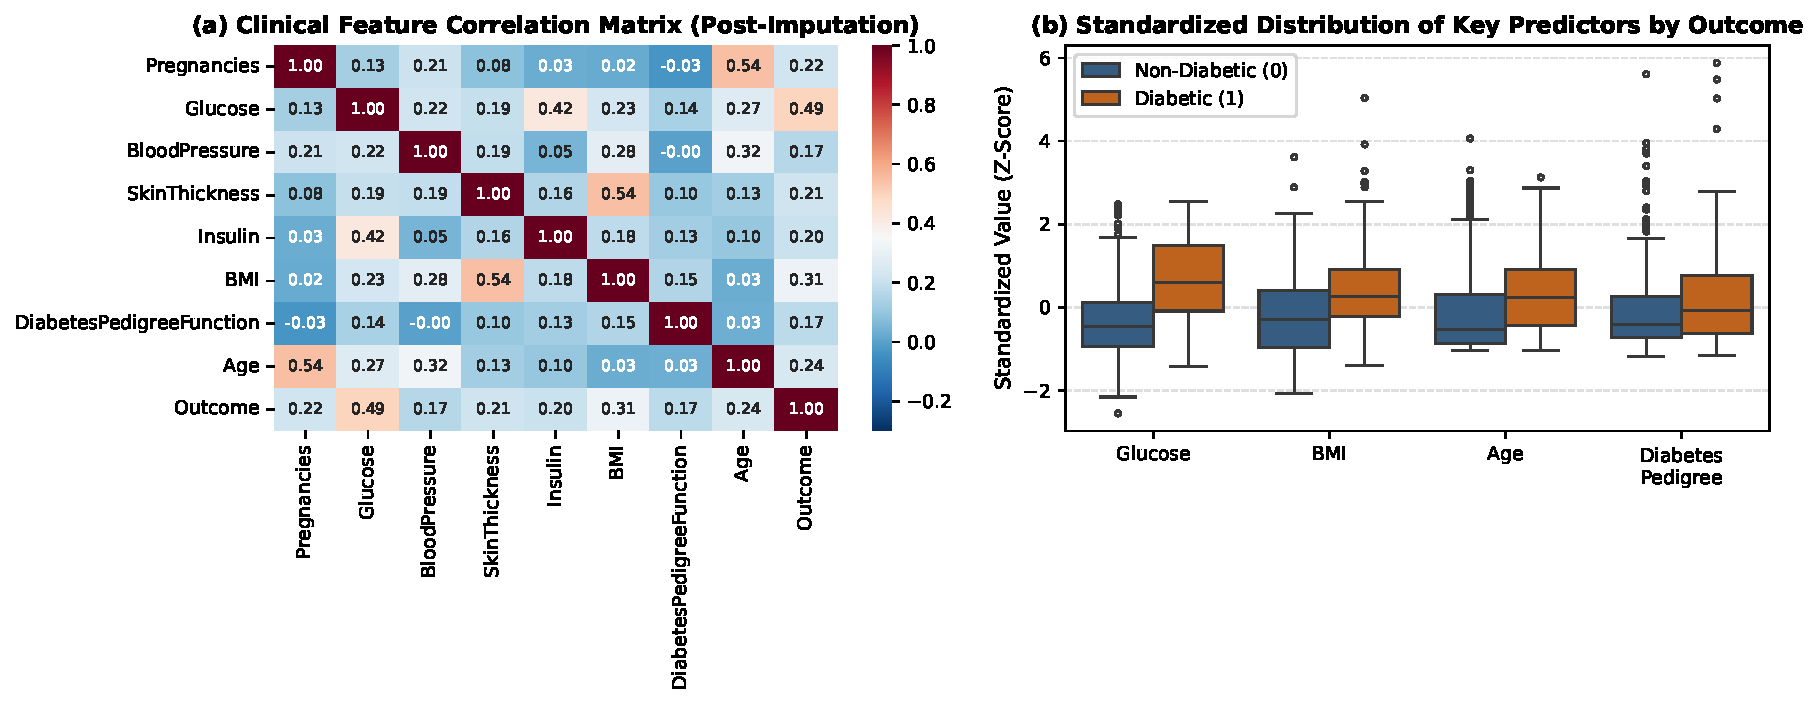
\includegraphics[width=0.86\textwidth]{../artifacts/figures/fig2_correlation_heatmap.pdf}
\caption{Clinical feature relationships post-imputation: (a) Pearson correlation matrix showing strong positive associations between \texttt{Glucose} and \texttt{Outcome} ($r = 0.49$), \texttt{BMI} and \texttt{SkinThickness} ($r = 0.54$), and \texttt{Age} and \texttt{Pregnancies} ($r = 0.54$); (b) standardized ($z$-score) boxplots of the four primary predictors stratified by diagnostic outcome.}
\label{fig:corr_box}
\end{figure*}

\subsection{Data Splitting and Zero-Leakage Preprocessing Pipeline}
To prevent any form of distributional or resampling leakage \cite{kaufman2012leakage, kapoor2023leakage}, the raw dataset $\mathcal{D}$ is immediately partitioned via an $80:20$ stratified train-test split ($\text{random\_state} = 42$):
\begin{itemize}
    \item \textbf{Training Partition ($\mathcal{D}_{\text{train}}$):} $n_{\text{train}} = 614$ patients ($400$ non-diabetic [$65.15\%$], $214$ diabetic [$34.85\%$]).
    \item \textbf{Held-Out Test Partition ($\mathcal{D}_{\text{test}}$):} $n_{\text{test}} = 154$ patients ($100$ non-diabetic [$64.94\%$], $54$ diabetic [$35.06\%$]).
\end{itemize}

All preprocessing transformations are encapsulated inside an \texttt{imblearn.pipeline.Pipeline} object so that parameters are estimated strictly from the active training fold $\mathcal{D}_{\text{train}}^{(k)}$ during 5-fold stratified cross-validation:
\begin{enumerate}
    \item \textbf{Biological Zero-to-NaN Recoding ($\Phi_{\text{zero}\to\text{NaN}}$):} A custom scikit-learn transformer replaces $x_{ij} = 0$ with \texttt{NaN} exclusively for $j \in \{\texttt{Glucose}, \texttt{BloodPressure}, \texttt{SkinThickness}, \texttt{Insulin}, \texttt{BMI}\}$.
    \item \textbf{Fold-Internal Median Imputation:} Missing entries in feature $j$ are replaced by the training-fold median $m_j^{(k)} = \text{median}(\{x_{ij} \in \mathcal{D}_{\text{train}}^{(k)} \mid x_{ij} \neq \text{NaN}\})$.
    \item \textbf{Z-Score Standardization:} Each feature is standardized using the training-fold mean $\mu_j^{(k)}$ and standard deviation $\sigma_j^{(k)}$:
    \begin{equation}
        \tilde{x}_{ij} = \frac{x_{ij} - \mu_j^{(k)}}{\sigma_j^{(k)}}.
    \end{equation}
    Standardization is essential for radial basis function (RBF) SVM margin computation and $k$-nearest neighbor distance metrics inside SMOTE.
    \item \textbf{Fold-Internal SMOTE (Experiments 2 and 3 only):} For each minority instance $\mathbf{x}_i \in \mathcal{D}_{\text{train},\text{min}}^{(k)}$, SMOTE selects one of its $k_{\text{nn}}$ nearest minority neighbors $\mathbf{x}_{zi}$ within the current training fold and synthesizes a new sample along the line segment \cite{chawla2002smote}:
    \begin{equation}
        \mathbf{x}_{\text{new}} = \mathbf{x}_i + \delta \cdot (\mathbf{x}_{zi} - \mathbf{x}_i), \quad \delta \sim \mathcal{U}(0, 1).
    \end{equation}
    During validation and test inference, the SMOTE step is automatically bypassed, ensuring that evaluation metrics are computed solely on authentic patient records.
\end{enumerate}

\subsection{Comparative Machine Learning Algorithms}
We evaluate four supervised classification algorithms representing distinct inductive biases:

\subsubsection{Decision Tree (CART)}
Classification and Regression Trees recursively partition the feature space by selecting split variables and thresholds that minimize node impurity, measured via the Gini index:
\begin{equation}
    G(t) = 1 - \sum_{c \in \{0,1\}} p(c \mid t)^2,
\end{equation}
or Shannon entropy $H(t) = -\sum_{c} p(c \mid t)\log_2 p(c \mid t)$. While fully grown decision trees provide transparent clinical rule paths, they possess unbounded capacity (low bias, extremely high variance) and readily overfit noisy clinical measurements unless constrained by maximum depth ($d_{\max}$), minimum leaf size ($n_{\text{leaf}}$), and cost-complexity pruning ($\alpha_{\text{ccp}}$).

\subsubsection{Random Forest (Bagging Ensemble)}
Proposed by Breiman \cite{breiman2001random}, Random Forest constructs an ensemble of $B$ decorrelated decision trees $\{T_b\}_{b=1}^B$ trained on bootstrap resamples of the training data, restricting each split search to a random subset of $m_{\text{try}} \le d$ features. By averaging predictions across diverse trees, Random Forest reduces variance relative to a single tree:
\begin{equation}
    \text{Var}\!\left(\frac{1}{B}\sum_{b=1}^B T_b(\mathbf{x})\right) = \rho \sigma^2 + \frac{1 - \rho}{B}\sigma^2,
\end{equation}
where $\rho$ denotes pairwise tree correlation and $\sigma^2$ is individual tree variance.

\subsubsection{Extreme Gradient Boosting (XGBoost)}
Developed by Chen and Guestrin \cite{chen2016xgboost}, XGBoost trains an additive ensemble of regression trees sequentially by minimizing a second-order Taylor expansion of the regularized binomial log-loss objective at iteration $t$:
\begin{equation}
    \mathcal{L}^{(t)} \approx \sum_{i=1}^{n} \left[ l(y_i, \hat{y}_i^{(t-1)}) + g_i f_t(\mathbf{x}_i) + \frac{1}{2} h_i f_t^2(\mathbf{x}_i) \right] + \Omega(f_t),
\end{equation}
where $g_i = \partial_{\hat{y}^{(t-1)}} l(y_i, \hat{y}_i^{(t-1)})$ and $h_i = \partial^2_{\hat{y}^{(t-1)}} l(y_i, \hat{y}_i^{(t-1)})$ are first- and second-order gradients, and $\Omega(f_t) = \gamma J + \frac{1}{2}\lambda \sum_{j=1}^J w_j^2$ explicitly penalizes the number of leaves $J$ and leaf weights $w_j$ ($L_2$ regularization $\lambda$).

\subsubsection{Support Vector Machine (SVM)}
Rooted in statistical learning theory \cite{cortes1995support}, soft-margin SVM seeks a maximum-margin separating hyperplane in a reproducing kernel Hilbert space induced by map $\phi(\mathbf{x})$:
\begin{equation}
    \min_{\mathbf{w}, b, \boldsymbol{\xi}} \frac{1}{2}\|\mathbf{w}\|_2^2 + C \sum_{i=1}^n \xi_i \quad \text{s.t. } y_i'(\mathbf{w}^\top \phi(\mathbf{x}_i) + b) \ge 1 - \xi_i,
\end{equation}
where $y_i' \in \{-1, +1\}$, $C > 0$ controls the penalty on margin violations $\xi_i \ge 0$, and the radial basis function (RBF) kernel is given by $K(\mathbf{x}_i, \mathbf{x}_j) = \exp(-\gamma \|\mathbf{x}_i - \mathbf{x}_j\|_2^2)$. Posterior class probabilities are calibrated via Platt scaling.

\subsection{Three-Stage Experimental Design and Tuning Protocol}
To systematically isolate the effect of class imbalance mitigation from structural hyperparameter optimization, we execute three sequential experimental stages across all four classifiers:
\begin{itemize}
    \item \textbf{Experiment 1 (Baseline):} Zero-leakage preprocessing ($\Phi_{\text{zero}\to\text{NaN}} \to \text{MedianImputer} \to \text{StandardScaler}$) paired with default classifier hyperparameters and natural class priors ($65.1\%$ vs.\ $34.9\%$).
    \item \textbf{Experiment 2 (Fold-Internal SMOTE):} Addition of SMOTE ($\text{sampling\_strategy} = 1.0$, $k_{\text{nn}} = 5$) strictly inside the training folds to balance the positive and negative classes ($400:400$ in the full training partition) while keeping default model hyperparameters.
    \item \textbf{Experiment 3 (Hyperparameter Tuning + Imbalance Optimization):} Joint optimization of SMOTE resampling parameters and classifier regularization hyperparameters using 5-fold stratified \texttt{GridSearchCV} on $\mathcal{D}_{\text{train}}$, maximizing cross-validated F1-score. Table~\ref{tab:hyperparams} reports the search grids and the optimal configurations selected on the training folds.
\end{itemize}

\begin{table*}[t]
\centering
\caption{Hyperparameter Search Grids and Optimal Configurations Selected via 5-Fold Stratified GridSearchCV (Experiment 3)}
\label{tab:hyperparams}
\begin{tabular}{p{2.2cm}p{7.4cm}p{5.5cm}r}
\toprule
\textbf{Classifier} & \textbf{Search Space Explored (GridSearchCV)} & \textbf{Optimal Hyperparameters Found} & \textbf{Best CV F1} \\
\midrule
Decision Tree & \texttt{criterion} $\in \{\text{gini}, \text{entropy}\}$, \texttt{max\_depth} $\in \{3, 4, 5, 6\}$, \texttt{min\_samples\_split} $\in \{10, 20, 30\}$, \texttt{min\_samples\_leaf} $\in \{5, 10, 15\}$, \texttt{ccp\_alpha} $\in \{0.0, 0.005, 0.01\}$, \texttt{smote\_ratio} $\in \{0.85, 1.0\}$ & \texttt{criterion}=\text{gini}, \texttt{max\_depth}=4, \texttt{min\_samples\_leaf}=15, \texttt{min\_samples\_split}=10, \texttt{ccp\_alpha}=0.0, \texttt{smote\_ratio}=1.0 & $0.6739 \pm 0.0246$ \\
\addlinespace[3pt]
Random Forest & \texttt{n\_estimators} $\in \{150, 250\}$, \texttt{max\_depth} $\in \{5, 7, 9\}$, \texttt{min\_samples\_split} $\in \{8, 12\}$, \texttt{min\_samples\_leaf} $\in \{3, 6\}$, \texttt{max\_features} $\in \{\text{sqrt}, 0.5\}$, \texttt{smote\_ratio} $\in \{0.85, 1.0\}$ & \texttt{n\_estimators}=250, \texttt{max\_depth}=7, \texttt{max\_features}=0.5, \texttt{min\_samples\_leaf}=3, \texttt{min\_samples\_split}=8, \texttt{smote\_ratio}=1.0 & $0.7112 \pm 0.0154$ \\
\addlinespace[3pt]
XGBoost & \texttt{n\_estimators} $\in \{100, 150\}$, \texttt{max\_depth} $\in \{2, 3, 4\}$, \texttt{learning\_rate} $\in \{0.03, 0.05, 0.1\}$, \texttt{subsample}=0.8, \texttt{colsample\_bytree} $\in \{0.8, 1.0\}$, \texttt{reg\_lambda} $\in \{1.0, 5.0\}$, \texttt{min\_child\_weight} $\in \{2, 5\}$, \texttt{smote\_ratio} $\in \{0.85, 1.0\}$ & \texttt{n\_estimators}=100, \texttt{max\_depth}=4, \texttt{learning\_rate}=0.03, \texttt{min\_child\_weight}=5, \texttt{reg\_lambda}=5.0, \texttt{subsample}=0.8, \texttt{colsample}=1.0, \texttt{smote\_ratio}=1.0 & $\mathbf{0.7121 \pm 0.0209}$ \\
\addlinespace[3pt]
SVM (RBF) & \texttt{C} $\in \{0.25, 0.5, 1.0, 2.0, 4.0\}$, \texttt{gamma} $\in \{\text{scale}, 0.03, 0.05, 0.08, 0.12\}$, \texttt{smote\_k\_neighbors} $\in \{3, 5, 7\}$, \texttt{smote\_ratio} $\in \{0.9, 1.0\}$ & \texttt{kernel}=\text{rbf}, \texttt{C}=0.5, \texttt{gamma}=0.03, \texttt{smote\_k\_neighbors}=5, \texttt{smote\_ratio}=1.0 & $0.6956 \pm 0.0091$ \\
\bottomrule
\end{tabular}
\end{table*}

\subsection{Evaluation Metrics and Bias--Variance Protocol}
Let $\text{TP}$, $\text{TN}$, $\text{FP}$, and $\text{FN}$ denote true positives, true negatives, false positives, and false negatives on $\mathcal{D}_{\text{test}}$. Because missing a diabetic patient ($\text{FN}$) delays clinical intervention whereas a false alarm ($\text{FP}$) triggers confirmatory laboratory testing, we report a comprehensive suite of complementary metrics:
\begin{align}
    \text{Accuracy} &= \frac{\text{TP} + \text{TN}}{\text{TP} + \text{TN} + \text{FP} + \text{FN}}, \\
    \text{Precision (PPV)} &= \frac{\text{TP}}{\text{TP} + \text{FP}}, \\
    \text{Sensitivity (Recall / TPR)} &= \frac{\text{TP}}{\text{TP} + \text{FN}}, \\
    \text{Specificity (TNR)} &= \frac{\text{TN}}{\text{TN} + \text{FP}}, \\
    \text{F1-Score} &= \frac{2 \cdot \text{Precision} \cdot \text{Sensitivity}}{\text{Precision} + \text{Sensitivity}}, \\
    \text{G-Mean} &= \sqrt{\text{Sensitivity} \times \text{Specificity}}.
\end{align}
Additionally, we compute threshold-independent Area Under the ROC Curve (ROC-AUC) and Area Under the Precision-Recall Curve (PR-AUC), along with $95\%$ non-parametric bootstrap confidence intervals ($1{,}000$ resamples). To diagnose overfitting (high variance) versus underfitting (high bias), we evaluate the train-to-test F1 generalization gap:
\begin{equation}
    \Delta F_{1,\text{test}} = F_{1,\text{train}} - F_{1,\text{test}}, \quad \Delta F_{1,\text{cv}} = \overline{F}_{1,\text{cv-train}} - \overline{F}_{1,\text{cv-val}}.
\end{equation}

\section{Results and Discussion}

\subsection{Baseline Performance and the Cost of Class Imbalance (Experiment 1)}
Table~\ref{tab:main_results} presents the complete quantitative benchmark across all 12 model-stage combinations, and Table~\ref{tab:cm_counts} details the exact confusion matrix counts and $95\%$ bootstrap confidence intervals on the held-out test set ($N = 154$: $100$ non-diabetic, $54$ diabetic).

In Experiment 1 (Baseline), all four classifiers exhibit a strong decision bias toward the majority non-diabetic class ($y = 0$). Specifically, baseline Random Forest and XGBoost achieve high Specificity of $0.8600$ ($86/100$ true negatives) and overall Accuracies of $0.7727$ and $0.7662$, respectively. However, their clinical Sensitivity (Recall) is severely constrained:
\begin{itemize}
    \item \textbf{Baseline Decision Tree} detects only $26$ of $54$ diabetic patients ($\text{Sensitivity} = 0.4815$, missing $28$ diabetic cases), yielding a dismal Test F1-score of $0.5149$ and ROC-AUC of $0.6357$.
    \item \textbf{Baseline SVM} detects $30$ of $54$ diabetic patients ($\text{Sensitivity} = 0.5556$, $\text{F1} = 0.6000$).
    \item \textbf{Baseline XGBoost and Random Forest} detect $32/54$ ($\text{Sensitivity} = 0.5926$, $\text{F1} = 0.6400$) and $33/54$ ($\text{Sensitivity} = 0.6111$, $\text{F1} = 0.6535$) diabetic patients, respectively.
\end{itemize}
This confirms the classic \emph{accuracy paradox} in medical screening: a baseline model achieving $77.27\%$ accuracy still fails to identify $38.89\%$ of diabetic individuals in the test cohort. Furthermore, all three unregularized tree models (Decision Tree, Random Forest, and XGBoost) achieve a perfect training score of $F_{1,\text{train}} = 1.0000$, producing massive train-to-test F1 generalization gaps ($\Delta F_{1,\text{test}} = 0.4851$ for Decision Tree, $0.3465$ for Random Forest, and $0.3600$ for XGBoost).

\begin{table*}[t]
\centering
\caption{Comprehensive Benchmark Results Across Experimental Stages on 5-Fold Stratified CV ($N=614$) and Hold-Out Test Set ($N=154$)}
\label{tab:main_results}
\resizebox{\textwidth}{!}{%
\begin{tabular}{llrrrrrrrrrr}
\toprule
\textbf{Stage} & \textbf{Algorithm} & \textbf{Train F1} & \textbf{CV F1 ($\mu \pm \sigma$)} & \textbf{CV AUC} & \textbf{Test Acc} & \textbf{Test Prec} & \textbf{Test Sens} & \textbf{Test Spec} & \textbf{Test F1} & \textbf{Test AUC} & \textbf{Gap $\Delta F_1$} \\
\midrule
\multirow{4}{*}{Exp 1: Baseline}
 & Decision Tree & $1.0000$ & $0.5518 \pm 0.0201$ & $0.6510$ & $0.6818$ & $0.5532$ & $0.4815$ & $0.7900$ & $0.5149$ & $0.6357$ & $+0.4851$ \\
 & Random Forest & $1.0000$ & $0.6330 \pm 0.0192$ & $0.8154$ & $\mathbf{0.7727}$ & $\mathbf{0.7021}$ & $0.6111$ & $\mathbf{0.8600}$ & $0.6535$ & $0.8181$ & $+0.3465$ \\
 & XGBoost       & $1.0000$ & $0.6117 \pm 0.0183$ & $0.7823$ & $0.7662$ & $0.6957$ & $0.5926$ & $\mathbf{0.8600}$ & $0.6400$ & $0.8057$ & $+0.3600$ \\
 & SVM (RBF)     & $0.7461$ & $0.6485 \pm 0.0187$ & $0.8333$ & $0.7403$ & $0.6522$ & $0.5556$ & $0.8400$ & $0.6000$ & $0.7964$ & $+0.1461$ \\
\midrule
\multirow{4}{*}{Exp 2: SMOTE}
 & Decision Tree & $1.0000$ & $0.6144 \pm 0.0100$ & $0.7012$ & $0.7013$ & $0.5690$ & $0.6111$ & $0.7500$ & $0.5893$ & $0.6806$ & $+0.4107$ \\
 & Random Forest & $1.0000$ & $0.6683 \pm 0.0356$ & $0.8208$ & $0.7532$ & $0.6333$ & $0.7037$ & $0.7800$ & $0.6667$ & $0.8139$ & $+0.3333$ \\
 & XGBoost       & $1.0000$ & $0.6063 \pm 0.0277$ & $0.7847$ & $0.7338$ & $0.6140$ & $0.6481$ & $0.7800$ & $0.6306$ & $0.8106$ & $+0.3694$ \\
 & SVM (RBF)     & $0.7930$ & $0.6854 \pm 0.0432$ & $0.8374$ & $0.7273$ & $0.5968$ & $0.6852$ & $0.7500$ & $0.6379$ & $0.8112$ & $+0.1551$ \\
\midrule
\multirow{4}{*}{Exp 3: Tuned+SMOTE}
 & Decision Tree & $0.7214$ & $0.6739 \pm 0.0246$ & $0.7926$ & $0.7662$ & $0.6324$ & $\mathbf{0.7963}$ & $0.7500$ & $\mathbf{0.7049}$ & $0.8012$ & $\mathbf{+0.0165}$ \\
 & Random Forest & $0.8358$ & $0.7112 \pm 0.0154$ & $0.8318$ & $0.7338$ & $0.5890$ & $\mathbf{0.7963}$ & $0.7000$ & $0.6772$ & $0.8146$ & $+0.1587$ \\
 & XGBoost       & $0.7531$ & $\mathbf{0.7121 \pm 0.0209}$ & $0.8385$ & $0.7338$ & $0.5915$ & $0.7778$ & $0.7100$ & $0.6720$ & $\mathbf{0.8224}$ & $+0.0811$ \\
 & SVM (RBF)     & $0.7043$ & $0.6956 \pm 0.0091$ & $\mathbf{0.8474}$ & $0.7273$ & $0.5882$ & $0.7407$ & $0.7200$ & $0.6557$ & $0.8078$ & $+0.0486$ \\
\bottomrule
\end{tabular}%
}
\end{table*}

\begin{table*}[t]
\centering
\caption{Hold-Out Test Set Confusion Matrix Counts, Geometric Mean, PR-AUC, and 95\% Bootstrap Confidence Intervals ($1{,}000$ Resamples)}
\label{tab:cm_counts}
\resizebox{\textwidth}{!}{%
\begin{tabular}{llrrrrrrll}
\toprule
\textbf{Stage} & \textbf{Algorithm} & \textbf{TN} & \textbf{FP} & \textbf{FN} & \textbf{TP} & \textbf{G-Mean} & \textbf{PR-AUC} & \textbf{Test F1 (95\% CI)} & \textbf{Test ROC-AUC (95\% CI)} \\
\midrule
\multirow{4}{*}{Exp 1: Baseline}
 & Decision Tree & $79$ & $21$ & $28$ & $26$ & $0.6167$ & $0.4482$ & $0.5149$ $[0.3830, 0.6286]$ & $0.6357$ $[0.5551, 0.7116]$ \\
 & Random Forest & $86$ & $14$ & $21$ & $33$ & $0.7250$ & $0.6989$ & $0.6535$ $[0.5306, 0.7563]$ & $0.8181$ $[0.7412, 0.8844]$ \\
 & XGBoost       & $86$ & $14$ & $22$ & $32$ & $0.7139$ & $0.6763$ & $0.6400$ $[0.5185, 0.7477]$ & $0.8057$ $[0.7282, 0.8759]$ \\
 & SVM (RBF)     & $84$ & $16$ & $24$ & $30$ & $0.6831$ & $0.6615$ & $0.6000$ $[0.4752, 0.7046]$ & $0.7964$ $[0.7195, 0.8659]$ \\
\midrule
\multirow{4}{*}{Exp 2: SMOTE}
 & Decision Tree & $75$ & $25$ & $21$ & $33$ & $0.6770$ & $0.4841$ & $0.5893$ $[0.4783, 0.6857]$ & $0.6806$ $[0.6026, 0.7557]$ \\
 & Random Forest & $78$ & $22$ & $16$ & $38$ & $0.7409$ & $0.6912$ & $0.6667$ $[0.5565, 0.7627]$ & $0.8139$ $[0.7401, 0.8803]$ \\
 & XGBoost       & $78$ & $22$ & $19$ & $35$ & $0.7110$ & $0.6679$ & $0.6306$ $[0.5172, 0.7308]$ & $0.8106$ $[0.7349, 0.8781]$ \\
 & SVM (RBF)     & $75$ & $25$ & $17$ & $37$ & $0.7169$ & $0.6728$ & $0.6379$ $[0.5242, 0.7288]$ & $0.8112$ $[0.7405, 0.8766]$ \\
\midrule
\multirow{4}{*}{Exp 3: Tuned+SMOTE}
 & Decision Tree & $75$ & $25$ & $\mathbf{11}$ & $\mathbf{43}$ & $\mathbf{0.7728}$ & $0.6440$ & $\mathbf{0.7049}$ $[0.6000, 0.7887]$ & $0.8012$ $[0.7189, 0.8688]$ \\
 & Random Forest & $70$ & $30$ & $\mathbf{11}$ & $\mathbf{43}$ & $0.7466$ & $0.6974$ & $0.6772$ $[0.5800, 0.7592]$ & $0.8146$ $[0.7403, 0.8770]$ \\
 & XGBoost       & $71$ & $29$ & $12$ & $42$ & $0.7431$ & $\mathbf{0.7125}$ & $0.6720$ $[0.5714, 0.7612]$ & $\mathbf{0.8224}$ $[0.7481, 0.8859]$ \\
 & SVM (RBF)     & $72$ & $28$ & $14$ & $40$ & $0.7303$ & $0.6937$ & $0.6557$ $[0.5487, 0.7392]$ & $0.8078$ $[0.7337, 0.8706]$ \\
\bottomrule
\end{tabular}%
}
\end{table*}

\subsection{Impact of Fold-Internal SMOTE Resampling (Experiment 2)}
Incorporating SMOTE strictly within the training folds (Experiment 2) shifts the classification boundary toward the minority class, yielding immediate gains in Sensitivity across all four algorithms:
\begin{itemize}
    \item \textbf{Decision Tree:} Sensitivity rises by $+12.96$ percentage points (from $0.4815$ to $0.6111$), lifting Test F1 from $0.5149$ to $0.5893$ and G-Mean from $0.6167$ to $0.6770$.
    \item \textbf{Random Forest:} Sensitivity improves by $+9.26$ percentage points (from $0.6111$ to $0.7037$), reducing false negatives from $21$ to $16$ and improving Test F1 to $0.6667$ and G-Mean to $0.7409$.
    \item \textbf{XGBoost:} Sensitivity increases from $0.5926$ to $0.6481$ (false negatives drop from $22$ to $19$) while Test ROC-AUC improves from $0.8057$ to $0.8106$.
    \item \textbf{SVM (RBF):} Sensitivity jumps by $+12.96$ percentage points (from $0.5556$ to $0.6852$), raising Test F1 from $0.6000$ to $0.6379$ and Test ROC-AUC from $0.7964$ to $0.8112$.
\end{itemize}
As expected from Bayes decision theory, equalizing the effective training priors trades off a modest fraction of Specificity (which shifts from $0.79$--$0.86$ in Exp 1 to $0.75$--$0.78$ in Exp 2) in exchange for substantial reductions in clinically hazardous false-negative diagnoses. However, SMOTE alone does not resolve the high variance of unconstrained tree estimators: Decision Tree, Random Forest, and XGBoost in Experiment 2 still exhibit $F_{1,\text{train}} = 1.0000$ and large generalization gaps ($\Delta F_{1,\text{test}} \in [0.3333, 0.4107]$).

\subsection{Hyperparameter Tuning and Multi-Metric Model Comparison (Experiment 3)}
Combining fold-internal SMOTE with 5-fold stratified hyperparameter optimization (Experiment 3) delivers significant improvements in both minority-class detection and generalization stability across all four paradigms (Fig.~\ref{fig:cm_grid} and Fig.~\ref{fig:stage_imp}(a)):
\begin{enumerate}
    \item \textbf{Tuned XGBoost:} Achieves the highest 5-fold cross-validation F1-score ($0.7121 \pm 0.0209$), the highest Test ROC-AUC ($0.8224$, $95\%$ CI $[0.7481, 0.8859]$), and the highest Test PR-AUC ($0.7125$). On the held-out test set, it correctly identifies $42$ of $54$ diabetic patients ($\text{Sensitivity} = 0.7778$, an increase of $+18.52$ percentage points over its baseline) while maintaining a Specificity of $0.7100$ ($\text{G-Mean} = 0.7431$, $\text{Test F1} = 0.6720$).
    \item \textbf{Tuned Random Forest:} Achieves the second-highest 5-fold CV F1-score ($0.7112 \pm 0.0154$) and high Test ROC-AUC ($0.8146$) and PR-AUC ($0.6974$). On the test partition, it captures $43$ of $54$ diabetic patients ($\text{Sensitivity} = 0.7963$, $\text{Specificity} = 0.7000$, $\text{Test F1} = 0.6772$, $\text{G-Mean} = 0.7466$).
    \item \textbf{Tuned Decision Tree:} Constraining tree growth to $\text{max\_depth} = 4$ and $\text{min\_samples\_leaf} = 15$ transforms the single CART classifier from the worst baseline model ($\text{Test F1} = 0.5149$) into the highest point-estimate Test F1 performer ($0.7049$, $\text{G-Mean} = 0.7728$), capturing $43$ of $54$ diabetic cases ($\text{Sensitivity} = 0.7963$) while preserving $75.00\%$ Specificity ($75/100$ true negatives) and boosting Test ROC-AUC from $0.6357$ to $0.8012$.
    \item \textbf{Tuned SVM (RBF):} Selecting $C = 0.5$ and $\gamma = 0.03$ produces the highest 5-fold CV ROC-AUC ($0.8474 \pm 0.0113$) and elevates Test Sensitivity to $0.7407$ ($40/54$ true positives, compared to $30/54$ at baseline) with $\text{Specificity} = 0.7200$, $\text{Test F1} = 0.6557$, and $\text{Test ROC-AUC} = 0.8078$.
\end{enumerate}

Fig.~\ref{fig:roc_pr} illustrates the Receiver Operating Characteristic (ROC) and Precision-Recall (PR) curves on the held-out test set. Across nearly the entire false-positive rate spectrum, Tuned XGBoost ($\text{AUC} = 0.822$) and Tuned Random Forest ($\text{AUC} = 0.815$) dominate the ROC envelope, while in the Precision-Recall plane---which is particularly sensitive to false-positive inflation under class imbalance---Tuned XGBoost achieves the highest integrated area ($\text{PR-AUC} = 0.709 / 0.7125$ average precision), substantially exceeding the no-skill prevalence baseline of $0.351$.

\begin{figure*}[t]
\centering
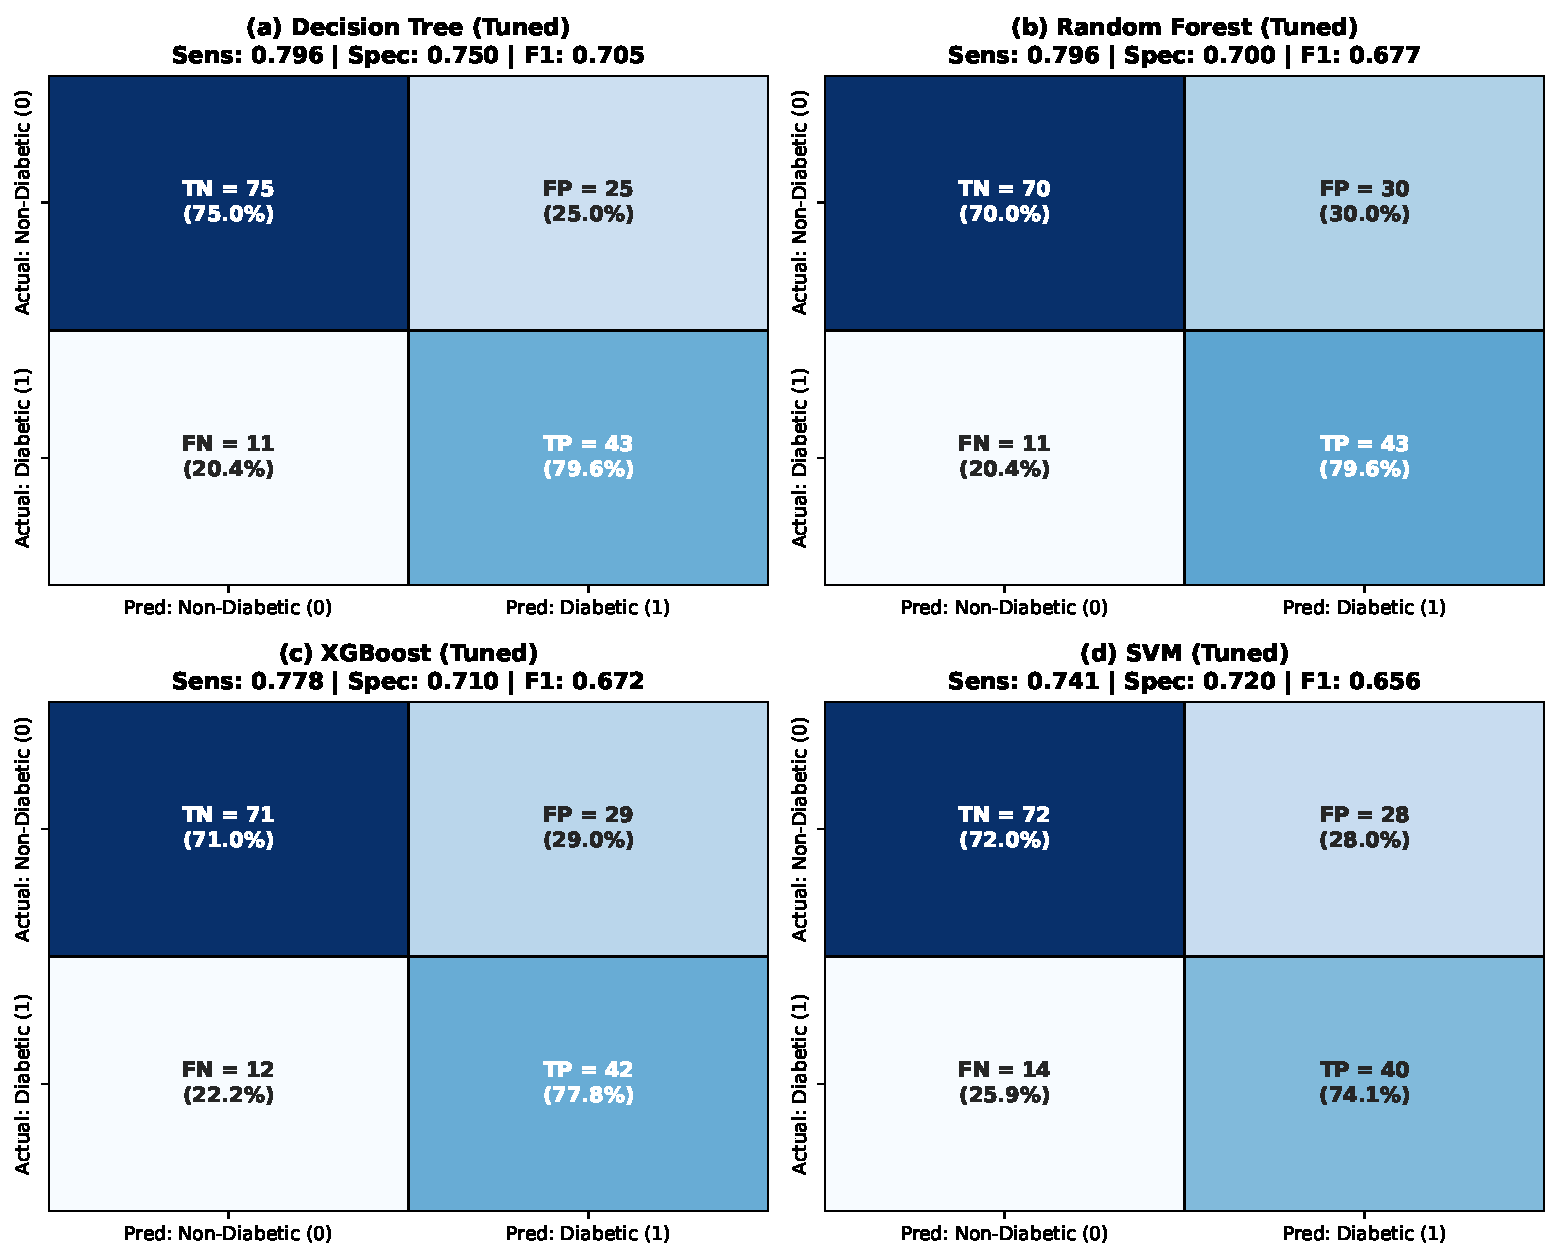
\includegraphics[width=0.76\textwidth]{../artifacts/figures/fig3_confusion_matrices.pdf}
\caption{Confusion matrices on the held-out stratified test set ($N = 154$: $100$ non-diabetic, $54$ diabetic) for the four tuned classifiers in Experiment 3: (a) Decision Tree, (b) Random Forest, (c) XGBoost, and (d) SVM (RBF). False negatives ($\text{FN}$) are reduced from $21$--$28$ in the baseline to $11$--$14$ after SMOTE and regularization tuning.}
\label{fig:cm_grid}
\end{figure*}

\begin{figure*}[t]
\centering
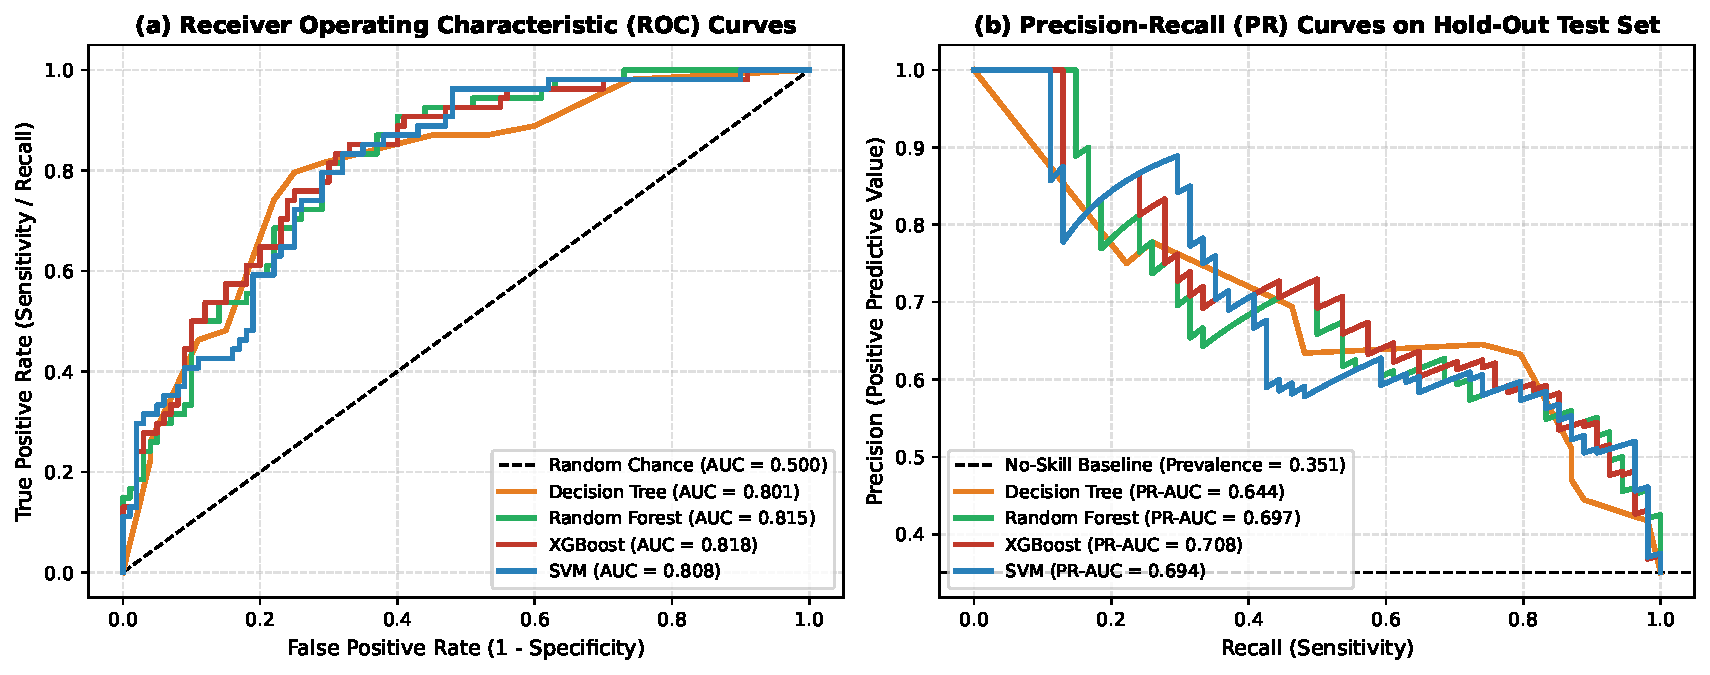
\includegraphics[width=0.84\textwidth]{../artifacts/figures/fig4_roc_pr_curves.pdf}
\caption{Threshold-independent discriminative comparison on the held-out test set ($N = 154$) for Experiment 3 models: (a) Receiver Operating Characteristic (ROC) curves showing Tuned XGBoost achieving the peak ROC-AUC of $0.822$; (b) Precision-Recall (PR) curves benchmarked against the $0.351$ prevalence baseline.}
\label{fig:roc_pr}
\end{figure*}

\subsection{Bias--Variance Trade-Off and Learning Curve Diagnosis}
A central requirement of rigorous experimental ML evaluation is diagnosing whether performance limitations stem from high variance (overfitting) or high bias (underfitting). Fig.~\ref{fig:learning_curves} depicts the 5-fold cross-validated learning curves (Training F1 vs.\ Cross-Validation F1 across training sample sizes from $n = 98$ to $n = 491$) for both the unadjusted Baseline models (Experiment 1, gray curves) and the Tuned models (Experiment 3, colored curves).

The learning curves reveal four key insights into the bias--variance dynamics of each algorithm:
\begin{enumerate}
    \item \textbf{Severe Variance in Unconstrained Decision Trees and Ensembles (Exp 1):} In Fig.~\ref{fig:learning_curves}(a)--(c), the baseline training F1-score remains pinned at the ceiling ($1.0000$) across all training sample sizes while the baseline cross-validation F1 plateaus around $0.55$--$0.63$. This persistent vertical separation ($\Delta F_{1,\text{cv}} = 0.4482$ for Decision Tree, $0.3670$ for Random Forest, and $0.3883$ for XGBoost) is the canonical signature of high variance: unconstrained trees partition the 8-dimensional feature space down to pure single-sample leaves, memorizing noise and imputed values rather than learning generalizable physiological thresholds.
    \item \textbf{Structural Pruning Eliminates Decision Tree Overfitting:} In Fig.~\ref{fig:learning_curves}(a), restricting the CART model to $\text{max\_depth} = 4$ and $\text{min\_samples\_leaf} = 15$ reduces the CV train-validation gap from $0.436$ to $0.057$ (and the full train-test gap $\Delta F_{1,\text{test}}$ from $0.4851$ to $0.0165$) while simultaneously raising the validation curve by $+12.2$ percentage points. This demonstrates that on small-to-moderate clinical tabular cohorts ($N < 1{,}000$) with noisy physiological features, aggressive capacity control shifts the estimator to a much healthier region of the bias--variance pareto frontier.
    \item \textbf{Shrinkage and $L_2$ Regularization in XGBoost vs.\ Bagging in Random Forest:} Comparing Fig.~\ref{fig:learning_curves}(b) and Fig.~\ref{fig:learning_curves}(c), Tuned Random Forest ($\text{max\_depth} = 7$, $\text{min\_samples\_leaf} = 3$) retains a moderate train-validation gap of $0.139$ ($\Delta F_{1,\text{test}} = 0.1587$), whereas Tuned XGBoost ($\text{max\_depth} = 4$, $\text{learning\_rate} = 0.03$, $\text{reg\_lambda} = 5.0$, $\text{min\_child\_weight} = 5$) compresses the CV gap to $0.061$ ($\Delta F_{1,\text{test}} = 0.0811$) while reaching the same high validation ceiling ($\sim 0.712$). Second-order gradient boosting with strong $L_2$ leaf weight penalty and conservative step size effectively prevents individual trees from chasing residual noise.
    \item \textbf{Low Variance and Smooth Margin Convergence in RBF SVM:} In Fig.~\ref{fig:learning_curves}(d), the RBF SVM exhibits the smallest variance across all stages. Reducing $C$ from $1.0$ to $0.5$ and setting $\gamma = 0.03$ widens the soft margin and smooths the Gaussian kernel radius, bringing the training and cross-validation curves into near-exact convergence ($\Delta F_{1,\text{cv}} = 0.006$, $\Delta F_{1,\text{test}} = 0.0486$) at $n = 491$. However, because the smooth RBF boundary cannot carve sharp axis-aligned thresholds on localized clinical interactions without increasing $\gamma$, its point-estimate test F1 ($0.6557$) trails the tree-based learners slightly.
\end{enumerate}

\begin{figure*}[t]
\centering
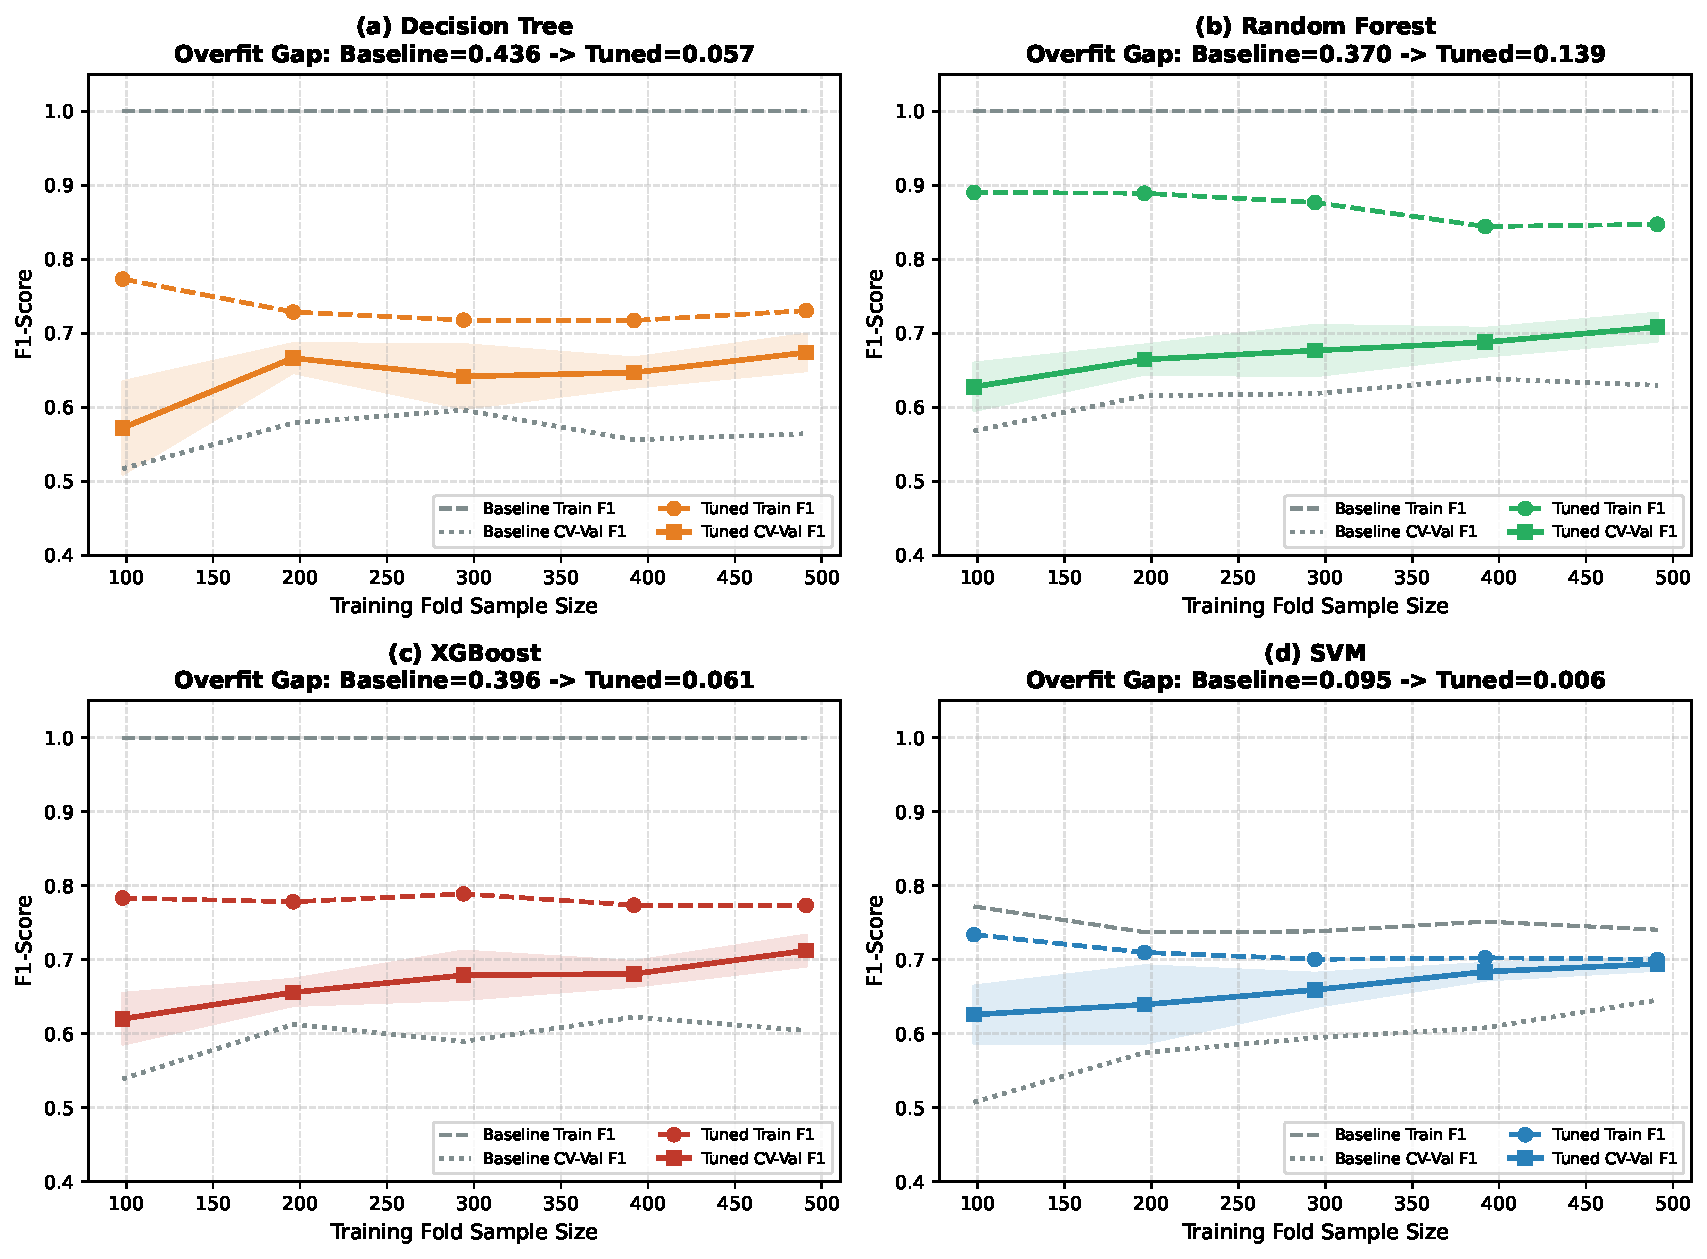
\includegraphics[width=0.78\textwidth]{../artifacts/figures/fig5_learning_curves_bias_variance.pdf}
\caption{Cross-validated learning curves (Training F1 vs.\ 5-Fold CV Validation F1 across training sample sizes) illustrating the bias--variance trade-off between Experiment 1 (Baseline, gray dashed/dotted lines) and Experiment 3 (Tuned+SMOTE, colored solid/dashed lines with $\pm 1\sigma$ shaded bands) for (a) Decision Tree, (b) Random Forest, (c) XGBoost, and (d) SVM.}
\label{fig:learning_curves}
\end{figure*}

\begin{figure*}[t]
\centering
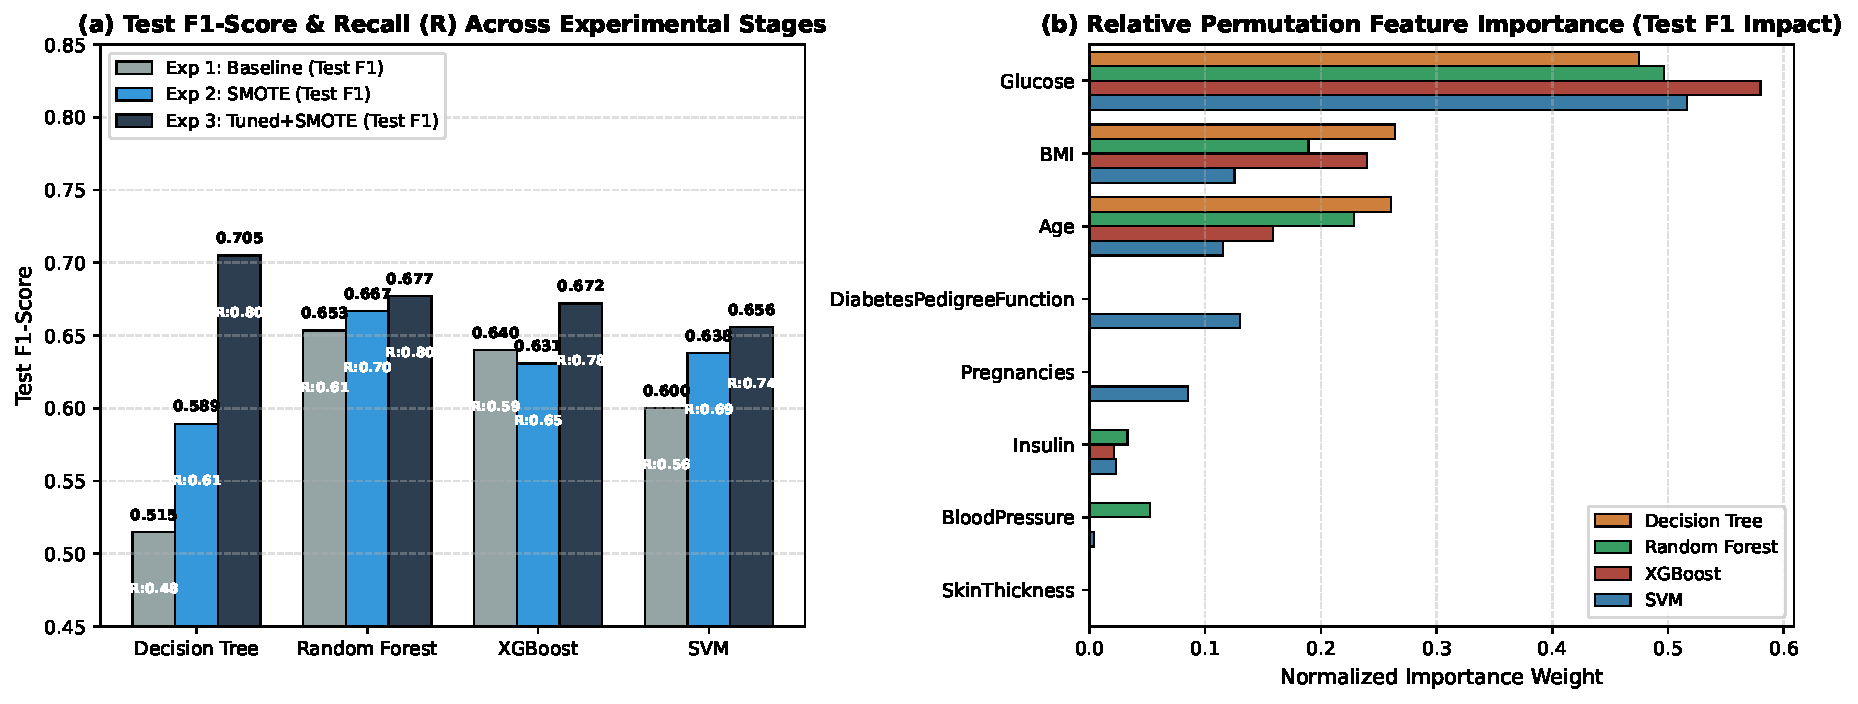
\includegraphics[width=0.84\textwidth]{../artifacts/figures/fig6_feature_importance.pdf}
\caption{Experimental progression and clinical feature attribution: (a) progressive improvement in Test F1-score and Sensitivity/Recall ($R$) across Experiment 1 (Baseline), Experiment 2 (SMOTE), and Experiment 3 (Tuned+SMOTE); (b) normalized permutation feature importance (Test F1 impact) demonstrating consensus across all four paradigms on \texttt{Glucose}, \texttt{BMI}, and \texttt{Age}.}
\label{fig:stage_imp}
\end{figure*}

\subsection{Clinical Feature Attribution and Optimal Model Selection}
To verify whether the learned decision rules align with established medical pathophysiology, Fig.~\ref{fig:stage_imp}(b) plots the normalized permutation feature importance (measured via decrease in Test F1 across $30$ random shuffles) for all four tuned models. Across every algorithmic paradigm, \textbf{Plasma Glucose Concentration} is the dominant predictor (accounting for $47.4\%$--$57.9\%$ of total permutation importance), followed consistently by \textbf{BMI} ($12.5\%$--$26.3\%$) and \textbf{Age} ($11.5\%$--$26.1\%$), with \textbf{Diabetes Pedigree Function} and \textbf{Pregnancies} contributing secondary discriminative signal in SVM and ensemble trees. This ranking is fully consistent with WHO diagnostic criteria, where post-load hyperglycemia (Glucose), visceral adiposity/insulin resistance (BMI), and age-related $\beta$-cell decline are the primary clinical drivers of T2DM \cite{smith1988using, zou2018predicting}. By contrast, \textbf{Skin Thickness} and \textbf{Insulin}---which suffered from $29.56\%$ and $48.70\%$ biological zero missingness, respectively---receive minimal permutation weight after median imputation, confirming that the regularized models appropriately avoid relying on heavily imputed attributes.

\textbf{Justification of Selected Optimal Model:} Selecting a single best model requires aligning statistical metrics with the clinical use case:
\begin{itemize}
    \item For \textbf{probabilistic risk ranking and clinical decision support integration}, \textbf{Tuned XGBoost} is selected as the primary recommended model. It achieves the highest 5-fold cross-validation F1-score ($0.7121 \pm 0.0209$), the highest Test ROC-AUC ($0.8224$), and the highest Test PR-AUC ($0.7125$), combined with strong Sensitivity ($0.7778$) and a well-controlled generalization gap ($\Delta F_{1,\text{test}} = 0.0811$). Because ROC-AUC and PR-AUC evaluate ranking fidelity across all operating thresholds, XGBoost provides clinicians with the most reliable calibrated risk probabilities.
    \item For \textbf{resource-constrained or rule-transparent point-of-care screening} where a fixed binary cutoff ($0.50$) and white-box interpretability are mandatory, the \textbf{Tuned Regularized Decision Tree} ($\text{max\_depth}=4$, $\text{min\_samples\_leaf}=15$) serves as an exceptional alternative, achieving the highest point-estimate Test F1 ($0.7049$), Sensitivity ($0.7963$), Specificity ($0.7500$), and G-Mean ($0.7728$) with virtually zero overfitting ($\Delta F_{1,\text{test}} = 0.0165$).
\end{itemize}

\subsection{Threats to Validity and Limitations}
Three limitations warrant consideration. First, the cohort is restricted to female patients of Pima Indian heritage, a population with a genetically and environmentally elevated prevalence of T2DM; external validation on multi-ethnic clinical registries is necessary before clinical deployment. Second, nearly half ($48.70\%$) of the 2-hour serum insulin values were unrecorded (encoded as zero); although fold-internal median imputation prevents data leakage, univariate imputation attenuates covariance with glucose. Third, the held-out test partition contains $N = 154$ patients ($54$ positives), resulting in $95\%$ bootstrap confidence intervals of roughly $\pm 0.08$ on F1 and $\pm 0.07$ on ROC-AUC (Table~\ref{tab:cm_counts}); thus, small single-split differences between Tuned Decision Tree, Random Forest, and XGBoost should be interpreted alongside their 5-fold cross-validation distributions.

\section{Conclusion}
This study presented a comparative experimental investigation of Decision Tree, Random Forest, XGBoost, and Support Vector Machine classifiers for early diabetes prediction on the Pima Indians Diabetes dataset under a strict zero-leakage preprocessing and resampling architecture. Our findings demonstrate three principal conclusions:
\begin{enumerate}
    \item Auditing and recoding biologically impossible zero values ($48.70\%$ in Insulin, $29.56\%$ in Skin Thickness, and $4.56\%$ in Blood Pressure) inside fold-isolated pipelines is essential to prevent data distortion and optimistic leakage.
    \item Unadjusted baseline classifiers suffer from the accuracy paradox under the $1:1.87$ class imbalance, yielding high specificity ($0.7900$--$0.8600$) but missing $38.89\%$--$51.85\%$ of diabetic patients ($\text{Sensitivity} = 0.4815$--$0.6111$) while exhibiting severe overfitting in unconstrained tree models ($\Delta F_{1,\text{test}} = 0.3465$--$0.4851$).
    \item Combining fold-internal SMOTE with stratified hyperparameter tuning boosts clinical Sensitivity to $0.7407$--$0.7963$ across all four models and compresses overfitting gaps below $0.16$. Tuned XGBoost delivers the most robust overall discriminative ranking ($\text{CV F1} = 0.7121$, $\text{Test ROC-AUC} = 0.8224$, $\text{PR-AUC} = 0.7125$), while a depth-constrained Decision Tree ($\text{max\_depth}=4$) achieves the highest binary threshold F1-score ($0.7049$) and G-Mean ($0.7728$) with direct clinical interpretability.
\end{enumerate}
Future work will investigate multivariate iterative imputation (MICE), cost-sensitive threshold moving tailored to clinical utility ratios, and SHAP-based patient-level explanations across multi-center electronic health record datasets.

\section*{Data and Code Availability}
To ensure full reproducibility, the self-contained Google Colab experimental notebook, modular Python source code, and raw benchmark outputs are publicly available in the companion repository and project deliverables archive.

\bibliographystyle{IEEEtran}
\bibliography{references}

\end{document}
